\chapter{Desarrollo de la Solución}
Dentro de esta sección se expone con precisión el procedimiento descrito previamente en la sección anterior, correspondiente a cada acción incluida en la metodología implementada, junto con los entregables previstos.

\section{Adquisición de los Datos}

\textbf{Actividad 1: Identificación de la data que contengan imágenes de rostros con características morfológicas faciales de proporciones similares}
 
Con el objetivo de entrenar un modelo de segmentación enfocado en características morfológicas faciales como arrugas y manchas, se llevó a cabo una exhaustiva búsqueda de bases de datos públicas en repositorios especializados. Se priorizó la recolección de conjuntos de datos que incluyeran imágenes faciales en alta resolución, variedad de edades, géneros y tonos de piel, así como condiciones de iluminación lo suficientemente controladas como para facilitar la segmentación de detalles faciales sutiles.

Durante este proceso, se identificaron diversos repositorios en plataformas como GitHub que ofrecían acceso a bases de datos con más de 200,000 imágenes faciales. Entre los conjuntos más destacados se encuentran versiones extendidas de datasets como CelebA, FFHQ (Flickr-Faces-HQ), y otros compendios curados por la comunidad investigadora, que contienen imágenes faciales etiquetadas o anotadas para tareas de reconocimiento y análisis facial.

Sin embargo, debido al enfoque específico de esta investigación la segmentación de características morfológicas finas como arrugas y manchas fue necesario realizar una selección cuidadosa de las imágenes más adecuadas. Para ello, se aplicaron criterios de claridad visual, resolución suficiente y visibilidad explícita de las deformaciones morfológicas faciales. Como resultado de este filtrado, se seleccionó un subconjunto compuesto por 5,000 imágenes faciales que cumplían con los siguientes criterios:

\begin{itemize}
    \item Alta calidad visual.   
    \item Visibilidad clara de texturas de la piel.
    \item Presencia evidente de arrugas y manchas.
    \item Proporciones faciales dentro de un rango estándar para facilitar el modelado.
\end{itemize} 

Este conjunto reducido pero representativo,lo podemos ver en la Figura \ref{4:fig1}, constituye la base de entrenamiento y validación del modelo propuesto. La selección manual de estos datos buscó optimizar el desempeño del modelo, al exponerlo exclusivamente a ejemplos que contienen información útil para aprender patrones asociados a las características morfológicas de interés.

\begin{figure}[h]
	\begin{center}
		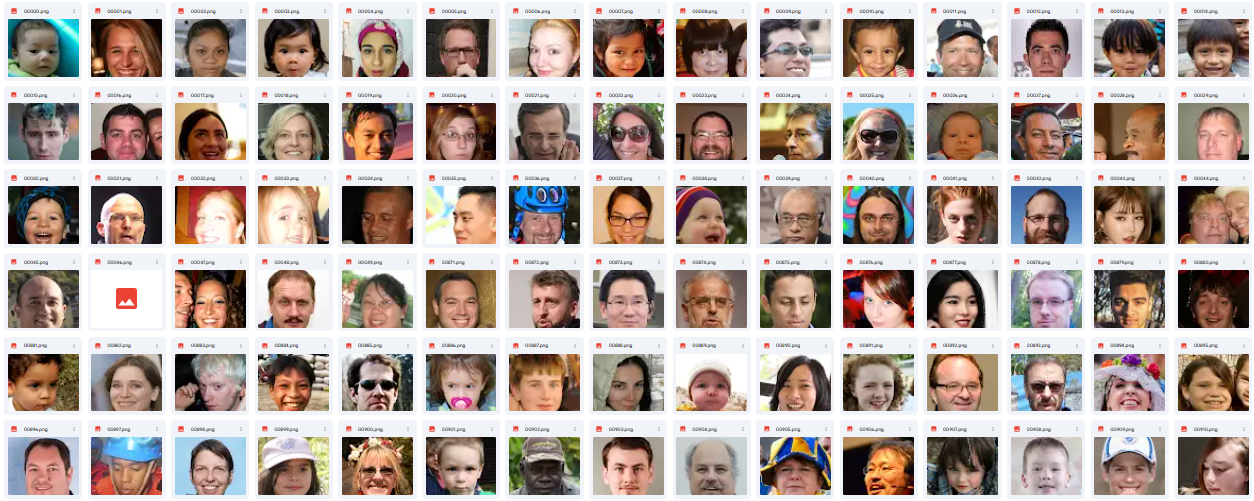
\includegraphics[width=0.75\textwidth]{4/figures/data.png}
		\caption[Dataset recolectado de repositorios]{Dataset recolectado de repositorios.\\
		Fuente: Elaboración propia}
		\label{4:fig1}
	\end{center}
\end{figure}

\section{Preprocesamiento de los Datos}

\textbf{Actividad 1: Filtración de imágenes faciales con características morfológicas}

Una vez recopilado el subconjunto de 5,000 imágenes faciales con características morfológicas visibles, se procedió a una etapa de filtración adicional orientada a reforzar la consistencia y la relevancia de los datos para la tarea de segmentación. Esta filtración se enfocó en garantizar que todas las imágenes seleccionadas contuvieran arrugas y manchas claramente identificables, descartando aquellas que, pese a su calidad visual, no presentaban estas características de manera explícita.

El proceso se realizó mediante una inspección semiautomática, apoyada en técnicas básicas de detección de texturas y realce de bordes para facilitar la identificación visual de las zonas con deformaciones. Como resultado, se aseguraron condiciones homogéneas entre las imágenes del dataset final, lo que permitió una base sólida para la generación de máscaras de segmentación precisas.

\textbf{Actividad 2: Representación y normalización de las imágenes faciales}

Con el conjunto de imágenes definitivo, se ejecutó un proceso de preprocesamiento estandarizado con dos objetivos principales: uniformar las dimensiones espaciales de las imágenes y generar las máscaras binarias asociadas a las regiones con deformaciones morfológicas.

En primer lugar, todas las imágenes fueron redimensionadas a una resolución uniforme de 1024x1024 píxeles, preservando la relación de aspecto y aplicando interpolación bilineal para mantener la calidad visual. Esta estandarización es fundamental para asegurar la compatibilidad estructural con las redes neuronales convolucionales utilizadas en etapas posteriores, y facilita la aplicación de operaciones convolucionales sobre áreas homogéneas.

En segundo lugar, se generaron máscaras binarias (en blanco y negro) correspondientes a cada imagen. Estas máscaras representan las regiones específicas del rostro que contienen arrugas, manchas u otras alteraciones morfológicas, codificadas de la siguiente manera:

\begin{itemize}
    \item Blanco (valor 1): Regiones con características morfológicas relevantes (objetivo de segmentación).   
    \item Negro (valor 0): Regiones sin interés morfológico.
\end{itemize} 

Las máscaras, como se ve en la Figura \ref{4:fig2}, fueron elaboradas a partir de una combinación de anotación semiautomática y herramientas de realce de texturas, contrastes y gradientes, con verificación manual en una muestra aleatoria para asegurar su validez.

\begin{figure}[h]
	\begin{center}
		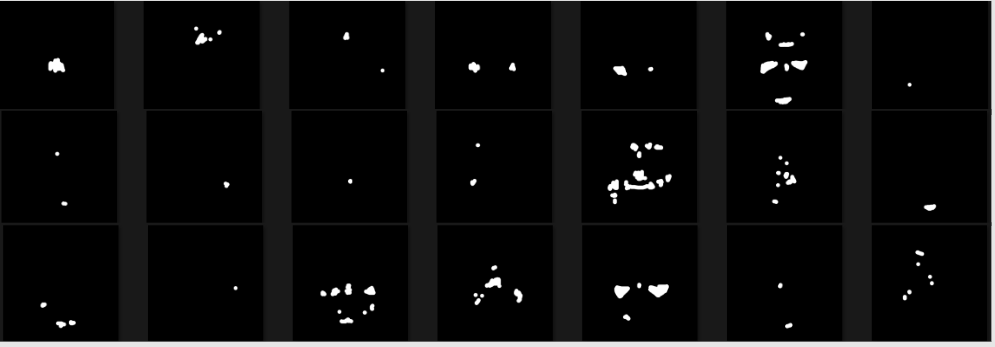
\includegraphics[width=0.75\textwidth]{4/figures/mascaras.png}
		\caption[Máscaras binarias generadas]{Máscaras binarias generadas.\\
		Fuente: Elaboración propia}
		\label{4:fig2}
	\end{center}
\end{figure}

Este proceso de representación y normalización, como se ve en el diagrama final de Preprocesamiento en la Figura \ref{4:fig3}, permitió convertir los datos originales en pares de entrada (imagen facial) y salida (máscara de segmentación), aptos para el entrenamiento supervisado del modelo de segmentación basado en redes neuronales convolucionales.

\begin{figure}[h]
	\begin{center}
		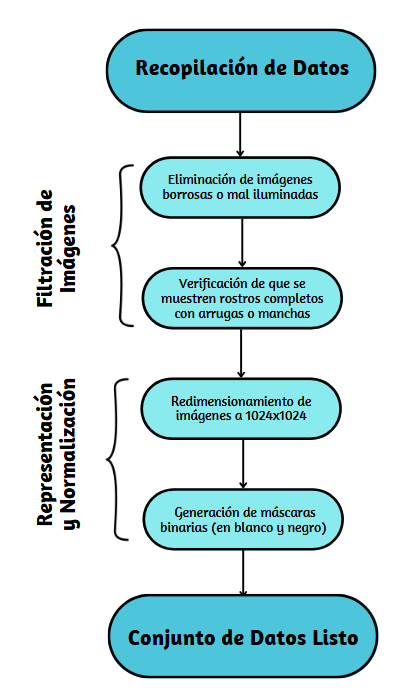
\includegraphics[width=0.75\textwidth]{4/figures/diagrama final prepo.png}
		\caption[Diagrama de Preprocesamiento Utilizado]{Diagrama de Preprocesamiento Utilizado.\\
		Fuente: Elaboración propia}
		\label{4:fig2}
	\end{center}
\end{figure}

\section{Desarrollo de los Modelos de Segmentación}

\textbf{Actividad 1: Diseño de la arquitectura del modelo}

\textbf{Actividad 2: Definición de componentes del modelo}

\textbf{Actividad 3: Estrategia de ensamblado del modelo}

\section{Entrenamiento del Modelo}

\textbf{Actividad 1: Configuración del entorno de entrenamiento}

\textbf{Actividad 2: Aplicación de técnicas de optimización}

\textbf{Actividad 3: Validación cruzada del rendimiento}

\section{Evaluación del Modelo}

\textbf{Actividad 1: Preparación de Datos de Validación}

\textbf{Actividad 2: Definición de Métricas de Evaluación}

\textbf{Actividad 3: Evaluación del Modelo}

\section{Despliegue}

\textbf{Actividad 1: Preparación del Entorno de Despliegue}

\textbf{Actividad 2: Despliegue del Modelo en Producción}
